%%
%%  Department of Electrical, Electronic and Computer Engineering.
%%  EPR400/2 Final Report - Proposal.
%%  Copyright (C) 2011-2016 University of Pretoria.
%%

This section contains the problem identification in the form of the complete
approved Project Proposal, unchanged from the final approved version.

\newpage

% Reset the section counter
\setcounter{section}{0}



%\import{proposal}

{
%\let\stdthebibliography\thebibliography
%\renewcommand{\thebibliography}{%
%  \let\section\subsection
%  \stdthebibliography}
%\begin{bibunit}[IEEEtran]

%\section{Problem statement}
%%
%%  Department of Electrical, Electronic and Computer Engineering.
%%  EPR400/2 Project Proposal - Section 1.
%%  Copyright (C) 2011-2018 University of Pretoria.
%%

\section{Problem statement}

\textbf{Motivation} \\
Shopping is a common chore for the average household\cite{Block:Shopping}. Before going shopping, a customer has to take note and write down their shopping list items one at a time, on a piece of paper. The customer then has to carry the shopping list everywhere they go, in case they need to do their shopping. The problem associated with this is that, since the list is written on a piece of paper, it is prone to being lost or forgotten at home, which leads to inconveniences when the customer wants to do their shopping. %A device has to be developed to account for t
%The present method of gathering shopping lists does not seem to be moving with the times of evolving technological advancements and is not secure from misplacing. Therefore the problem to be taken care of is to develop a system that is more efficient in how it assists users with gathering their shopping lists.
\noindent
\\\\
\textbf{Context} \\
%Everyone needs to do their shopping once in a while.
%A device should be produced as the end-product to the customer. The device shall be able to assist the customer with their shopping. The customer writes their shopping list on the device while at home and the list is automatically saved within the device, while the customer is writing the list. When the customer is shopping and realizes that they need the list, it should be sent to them, at the click a button that requests the list.
The best methods of solving a problem like this involve integration of home-based automation systems and control systems\cite{Kuo:Automatic_Control_Systems}, with devices being controlled by instructions from the user\cite{Yuksekkaya:Automation_Systems}.
%The customer currently writes their shopping list on a piece of paper, one item after another. The customer then has to carry the shopping list everywhere they go, in case they need to do their shopping. Since the list is written on a piece of paper, it will be prone to being lost, which is a major inconvenience.
A solution that has been tried before to ensure that lists do not get lost, is that of saving a screenshot of the customer's list, on their phone\cite{WinNT}. This solution is not desirable due to the fact that the customer cannot then cross things off their list if they change their mind. Another solution currently in use is that of using the Android application called "ShopList"\cite{ShopL}. The biggest drawback is that it is not flexible enough to add items which are not recognized internally by the program. In addition, the shopping list items can only be recorded by the phone's owner, not other members of the household.\\
The device to be produced to address the problem statement will be a great improvement on these methods because the customer can add any items of their choice to the shopping list and will be able to edit the list as they please. In addition to what has been mentioned, unlike the piece of paper where the shopping list is commonly  written on, the device will be attached to the customer's fridge with no chance of being lost. Also, the customer will not have to worry about losing their shopping list because it will always be with them at the tip of a button on their smartphone. The device to be produced also provides the functionality for other members of the household to add items onto the shopping list, unlike shopping applications like ShopList\cite{ShopL}.
\noindent
\\\\
\textbf{Technical Challenge} \\
% engineering challenge is to design and develop a device that takes the customer's shopping list input in handwritten form and saves it so that when the customer requires it, they will only have to press a button on their phone, and the device will send it to them. The engineering aspects of the project are as follows:
The engineering challenges associated with the project are to: (i) develop a small device that operates on a nonchargeable battery power supply, (ii) design and implement a text recognition algorithm to scan the user's input and convert it to recognizable text, (iii) design and implement a communication protocol to enable the device to send messages to the customer's smartphone wherever they are and (iv) design a mobile application that enables the user to obtain their shopping list from the device at home by clicking a single button. \\\\
\noindent
\textbf{Limitations}\\
The mobile application to be used to obtain the shopping list will run on smartphones using the Android Operating System only. Furthermore, the accuracy of the handwriting recognition software will be limited by the Optical Character Recognition code and the neural networks developed for that specific code. Since the customized micro-electronic components cannot be prototyped, the developer will be limited to use low cost components to build the system.
\nocite{Haykin:Communication_Systems}

%% End of File.

%%
%%  Department of Electrical, Electronic and Computer Engineering.
%%  EPR400/2 Project Proposal - Section 2.
%%  Copyright (C) 2011-2018 University of Pretoria.
%%

\section{Project requirements}

\subsection{Mission requirements of the product}
Specific details of the mission requirements of the product are listed below.
\begin{itemize}
	\item The user should get their shopping list sent to their phone from the device when they request for it.
	\item A small portable device must be produced.
	\item The device should run on non-rechargeable batteries.
	\item The device should contain a battery meter and should warn the user when the battery is low.
	\item The produced device must scan input from a user's handwriting and convert it to recognizable text.
	\item The device should display the list in recognizable and readable font.
	\item The produced device must automatically save what is written on its screen, in case the battery dies out.
	\item The user should use a touch-pen to write their shopping list items onto the touchscreen, which saves them into the device's memory.
\end{itemize}
\subsection{Student tasks}
The steps listed below need to be taken for mission requirements to be met.
\begin{itemize}
	\item A program must be developed for a smartphone so that it can request a document from the produced device.
	\item A communication interface must be established between the user's smartphone and the produced device.
	\item A handwriting recognition system must be implemented for conversion from user handwriting to recognizable text. 
	\item A magnetic casing should be designed for the device so that it can be attached to a fridge.
	%\item A program must be developed to capture the information from the touchscreen, either screen-shot capture or text capture.
	\item A polling and timing algorithm should be implemented so that after a specific amount of time, the contents on the touchscreen are automatically saved.
\end{itemize}
\newpage

\newpage

%% End of File.




%%
%%  Department of Electrical, Electronic and Computer Engineering.
%%  EPR400/2 Project Proposal - Section 3.
%%  Copyright (C) 2011-2018 University of Pretoria.
%%

\section{Functional analysis}
The breaking down of the system into functional sub-components is shown in Figure 1.
\begin{figure}[h]
	\centering
	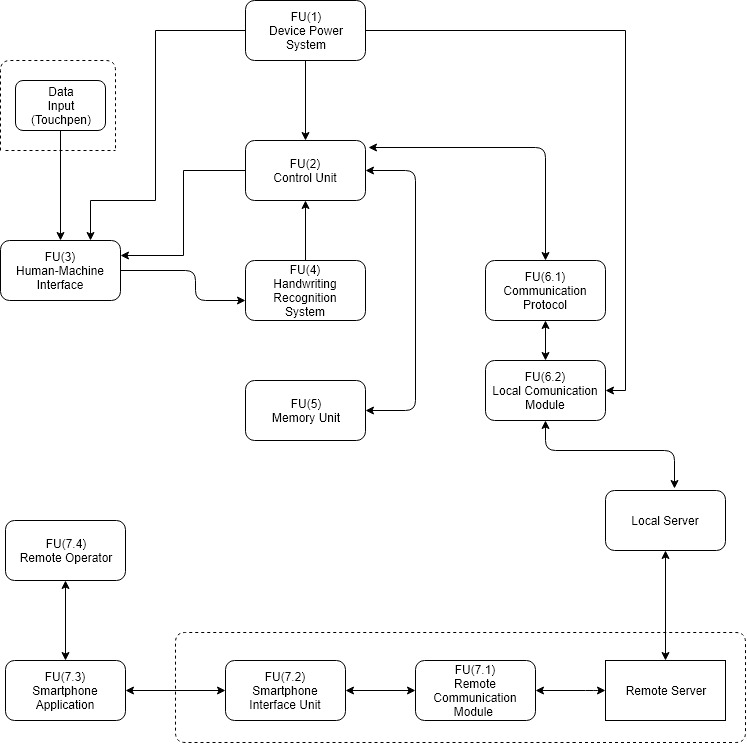
\includegraphics[scale=0.63]{blockchan.jpg}
	\caption{Functional Block diagram of the system to be developed.}
\end{figure}
\clearpage
\noindent
FU1, the device power system supplies power to the embedded control unit, FU2, which controls the whole system on the device. It also powers the modules that are responsible for the wireless transmission of the user's shopping list to their smart-phone, FU6.2. \\
All processes that happen on the device go through FU2. It is the root of the device, in other words if it breaks down, the whole system will not work and if it is faulty, the whole system will be faulty. Therefore, debugging mainly starts from FU2, to the other sub-components dependent on it.\\
FU3, the human-machine interface, is responsible for inputting the user's shopping list to the control unit in their own handwriting. It also displays the output received from the control unit. There is direct interaction with the user acting as the local operator.\\
Handwriting input from the user is converted to readable text, via FU4, the handwriting recognition system. A timer system is implemented within the system so that after a specific amount of time, data on FU3 is passed to FU4, which scans the data and compares it to a initially trained data set within FU4 and outputs the string that is learned from the data set. The recognition and learning process is implemented by use of back-propagating neural networks.\\
The inputs from FU3 will be words that will be on a line on FU3. A word segmentation algorithm is used to split each word into characters by use of the spaces between the handwritten characters that make up each handwritten word. The segmentation algorithm also contains a way to recognize space between full words that are input by the touch-pen onto FU3. This space is larger than the space between characters. Each raw input letter that is obtained after segmentation is then converted to the nearest learned text letter using the handwriting recognition algorithm. The converted letters are then concatenated after conversion of every letter on the line, to form the full words contained in the input line, in text. In the process of full-word integration, comparisons are made between succeeding characters to determine if they make grammatical sense next to each other. If not, the user is given the option to enter these words again, and if the learned words are the same, a suggestion for possible intended characters is displayed, with the user being given the option to keep the characters they entered or correct their input with the suggestions. The line containing the converted words with spaces between them, in text format, is displayed on the upper part of FU3 and the user inputs the next line onto the bottom part of FU3 that prompts for the user's next shopping item data input. The input line of handwritten text is converted to text using the previously defined method and the output is appended to the line after the previously converted line. This process continues until the user enters their full shopping list. \\
After FU4 successfully converts the user's shopping list input, the training data is updated with the input data that will just have been successfully converted. The training data is updated in a First-In First-Out manner with the assumption that the training data just obtained will most likely look like the data input to be input in the near future.  
FU4 passes the converted text to FU2, the control unit so that the text is saved to the memory of the system, FU5. \\
Information is sent to the user's smart-phone through FU6.1, the communication protocol. The user's phone has an in-built communication system, FU7.2 which interacts with FU6.1, the local communication module of the device. The shopping list input by the local operator is obtained on the smart-phone via FU7.3, the smart-phone application. The user requests the shopping list via the remote operator, FU7.4 which controls FU7.3.
\clearpage
\newpage

%% End of File.



\section{Target Specifications}

\subsection{Mission-critical system specifications}
\begin{center}
	\begin{longtable}{|p{5cm}|p{5cm}|p{5cm}|}
		\hline
		\textbf{SPECIFICATION} &
		\textbf{ORIGIN} &
		\textbf{VERIFICATION}\\
		\hline
		Information should be sent at request, to the mobile phone within 10 seconds.
		&
		The customer needs the shopping list sent to them as quickly as possible, but accounting for internet downtime, firewalls and wireless signal strength, there are going to be delays in the transmission path.
		&
		A timer will be programmed within the mobile application to track the time taken between a  request for the shopping list and when it is received.
		\\
		\hline
		Accuracy of the handwriting character detection must be greater than 80$\%$.
		&
		A trade-off has to be made between conversion time and performance or accuracy. Additionally, with optimizing conversion time comes the downside of more cost since the processor memory for the conversions has to be increased.
		&
		Error rate calculation will be displayed every time a word is updated. \\
		% \hline
		% The device should send and receive information to a smartphone $\geq$5m away
		%    &
		% The device should interface with the smart-phone in a wireless manner %and thproves the two devices can communicate if one of them is anywhere in the city, provided there is consistent network access.
		%    &
		% Send a random text file from the device to the cellphone.
		%    \\
		\hline
		The system should recognize that the user has completed writing their shopping list.
		&
		Character recognition should start as soon as the user finishes writing their line in their handwriting to prevent the user from waiting for too long. Therefore if it is known that writing is complete, the recognition process can easily be triggered by a boolean flag.
		&
		A flashing white LED will be switched on 1 second after data input is finished.
		\\
		\hline
		The user must be warned when the battery power remaining is less than $10\%$ of full capacity.
		&
		The device has be on so that the list can be sent to the user's phone when they request for it.
		& 
		A red LED will flash on the device when the battery power is less than $10\%$.\\
		\hline
		Handwritten input must be converted to text by the character recognition software in less than 1s.
		&
		The user has to see if the converted text has errors and correct them as soon as possible before proceeding too far ahead with their text input process.
		& 
		An LED will be configured to switch on as long as conversion is not complete.\\
		\hline
		Text recognition should consider the probability of occurance of combinations of letters.
		&
		This reduces grammatical errors in the shopping list and reduces the search pool for the conversion of the next letter, reducing search time for the goal node containing the equivalent letter in the neural network.
		& 
		The device's touchscreen should display suggestions for consecutive characters that are converted to text but do not make grammatical sense next to each other.\\
		\hline
		The communication link between the device's communication system and the phone system should transfer data bidirectionally, at a rate of between $5 \textrm{Mbps}$ and  $10 \textrm{Mbps}$ so that the bit error rate can be less than 10$\%$. 
		& 
		The device should send the shopping list to the user's smart-phone at any mall in the city. A balance has to be found in the transmission rate because if the rate is too fast, the rate at which errors are generated during transmission increases, meaning the transmitted shopping list data will not be reliable with some letters being missed during transmission. However, if the speed is too low, then the user will be left waiting too long in the store for their shopping list to be delivered to them before they start doing their shopping.
		&
		Using linear programming methods to calculate the data transmission rate and display it on the touchscreen of the shopping list device \cite{Shannon:A_Mathematical_Theory_of_Communications}.\\
		\hline
		\caption{Mission-critical system specification}
	\end{longtable}
\end{center}
\newpage
\subsection{Field conditions}
\begin{center}
	\begin{longtable}{|p{7.5cm}|p{7.5cm}|}
		\hline
		\textbf{REQUIREMENT} &
		\textbf{SPECIFICATION} \\
		\hline
		The device should read handwriting input from multiple users. 
		&
		There will be more than 2 training sets for the handwriting recognition neural network that will be useful for conversion of handwritten data to text.   
		\\
		\hline
		The device should operate under varying light conditions that will be typical of what the user will encounter in indoor environments.
		&
		The device operates in a light intensity in the range of 50 lux  to 1000 lux.
		\\
		\hline
		
		\caption{Field conditions}
	\end{longtable}
\end{center}
\newpage
%% End of File.
%%
%%  Department of Electrical, Electronic and Computer Engineering.
%%  EPR400/2 Project Proposal - Section 5.
%%  Copyright (C) 2011-2018 University of Pretoria.
%%

\section{Deliverables}

\subsection{Technical deliverables}

\begin{center}
	\begin{longtable}{|p{7cm}|p{3.5cm}|p{3.5cm}|}
		\hline
		\textbf{DELIVERABLE} & \textbf{DESIGNED AND IMPLEMENTED BY STUDENT} &
		\textbf{OFF-THE-SHELF} \\
		\hline
		Optical character recognition algorithm for handwritten input to text conversion. The algorithm will be implemented on the hand-held shopping list device.  It contains the segmentation code for separating the handwriting input as well as the exception code for consecutive characters that should not be next to each other.&     X&  \\
		\hline
		Touchscreen for the user to write their handwriting input of their shopping list onto the shopping list device. It will also display the converted text from the optical character recognition software. The touchscreen will be part of the hand-held shopping list device.       &     & X \\
		\hline
		Mobile application on the user's cellphone to get the shopping list, saved on the shopping list device at home, sent onto the cellphone.         &   X  &  \\
		\hline
		Touch-pen used by the user to enter their handwritten shopping list items on the shopping list device's touchscreen. & & X\\
		\hline
		GSM module for the shopping list device's communication system so that commands can be received and information can be sent to the user's phone.& & X\\
		\hline
		Embedded processor board for the shopping list device's control unit.  & & X\\
		\hline
		Integration of the embedded processor board, the GSM modules and the LCD touchscreen to make the shopping list hardware device.  & X& \\
		\hline
		Assembly/C-Code to connect the Wi-Fi modules to the embedded system's serial ports and set-up a wireless connection.& X& \\
		\hline
		\caption{Deliverables}
	\end{longtable}
\end{center}

\subsection{Demonstration at the examination}
1. The demonstration will commence with the user pressing the device's power button. An option will be available for the user to write their list.\\
2. The demonstrator will then write a number of sentences on the touchscreen of the device and wait for them to be converted to text.\\
%2. The demonstrator will then write on the touchscreen of the device, a number of sentences and wait for them to be converted to text.\\
3. The demonstrator will then start up the Android application on the mobile phone. \\
4. The demonstrator will then press the button on the Android application interface, that requests the shopping list from the device.\\
5. The application will then display on the screen of the smartphone, the list of sentences that was put in by the demonstrator onto the touchscreen of the device in stage 2 of the demonstration.\\
\newpage

\bibliographystyle{IEEEtran}
\appto{\bibsetup}{\raggedright}
\bibliography{proposal}


%\putbib[proposal]
%\end{bibunit}
%}

% Reset the section counter
\setcounter{section}{0}

\newpage

%% End of File.

